%========================================================================================================================
%========================================================================================================================
%========================================================================================================================
\section{Semantics}
\label{sec:semantics}
In this section, we present the consistency enforcement mechanism of
\tool, abstracted as a formal operational semantics. Our approach is
complete for the specification language defined in
Sec.~\ref{sec:ctrt_language}, however for better
comprehensibility, here we present the semantics and the theorems
paramterized over a non-hybrid contract consisting of one proposition.
Therefore, in the rest of this section, we will assume a given contracat $\psi$
of the following form:
\begin{fmathpar}
\begin{array}{lll}
\psi = \forall a. a \xrightarrow{\rel_1;\rel_2;...;\rel_k} \hat{\eta} \Rightarrow a 
\xrightarrow{\visZ} \hat{\eta}
&\qquad 
\quad & \rel_i \in \{\visZ;\soZ\}
\end{array}
\end{fmathpar}
%
%

The operational semantics is defined via a small-step relation over \emph{execution
states}, which are tuples of the form $\E=(\EffSoup,\visZ ,\soZ)$.
The \emph{effect soup} $\EffSoup$, stands for the set of all
effects produced in the system, and \emph{primitive relations} $\visZ$,
$\soZ$ $\subseteq \EffSoup \times \EffSoup$, respectively represent the
visibility and session order 
among such effects. Figures \ref{subfig:execution_graph} and
\ref{subfig:execution_example} represent a simple
execution state consisting of 9 effects with associated
primitive relations\footnote{we ommit drawing transitive $\soZ$
edges (e.g. between
$\eff_8$ and $\eff_1$) for better readability}.
\begin{figure}[h]
	
	\begin{subfigure}[b]{0.28 \textwidth}
	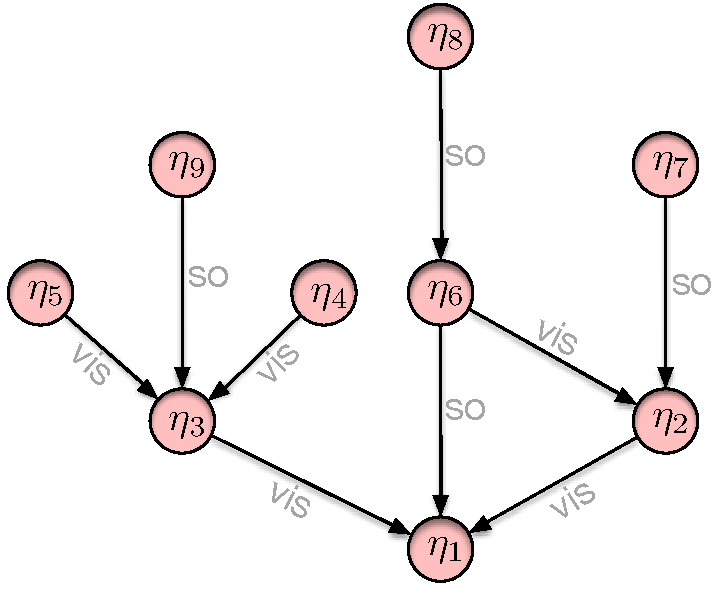
\includegraphics[scale=0.38]{Figures/execution.pdf}
	\subcaption{An execution state \E}
	\label{subfig:execution_graph}
	\end{subfigure}
	%
	\quad \vrule \quad
	%
	\begin{subfigure}[b]{0.31 \textwidth}
	\begin{smathpar}
	\begin{array}{lcl}
	\E.\EffSoup & = & 
	\{\eta_1,\eta_2,\eta_3,\eta_4,\eta_5,\eta_6,\eta_7,\\ & & \;\eta_8,\eta_9\}\\
	\E.\visZ & = & 
	\{(\eta_5,\eta_3),(\eta_4,\eta_3),(\eta_3,\eta_1),\\ &
	&\;(\eta_2,\eta_1),(\eta_6,\eta_2)\} \\ 
	\E.\soZ & = & \{(\eta_9,\eta_3),(\eta_8,\eta_6),(\eta_6,\eta_1),\\ 
	& & \;(\eta_8,\eta_1),(\eta_7,\eta_2) \} \\ 
	\end{array}
	\end{smathpar}\\
	\subcaption{Effect soup and primitive relations}
	\label{subfig:execution_example}
	\end{subfigure}
	%
	\quad \vrule \quad
	%
	\begin{subfigure}[b]{0.3 \textwidth}
	\begin{smathpar}
	\begin{array}{lll}
	\visZ^{-1}  (\eta_1) & = & \{\eta_2,\eta_3\} \\ 
	\soZ^{-1}  (\eta_1) & = & \{\eta_6, \eta_8\} \\
	(\soZ\cup\visZ)^{-1} (\eta_1) & = &
	\{\eta_2,\eta_3,\eta_6,\eta_8\} \\ 
	(\visZ^*)^{-1} (\eta_1) & = &
	\{\eta_2,\eta_3,\eta_4,\eta_5,\eta_6\} \\ 
	(\soZ;\visZ)^{-1}(\eta_1) & = & \{\eta_7,\eta_9\}
	\\ \\
	\end{array}
	\end{smathpar} \\
	\subcaption{Relation inverse examples}
	\label{subfig:inverse_example}
	\end{subfigure}
	\caption{A simple execution state }
\label{fig:execution_state}
\end{figure}

We denote the subset of $\EffSoup$ consisting of effects that
satisfy a certain condition as $\EffSoup_{(\mathtt{condition})}$.
%

Note that \tool's contracs are in fact constraints over execution states,
where the domain of quantification is fixed to the effect soup
$\EffSoup$, and
interpretation for $\soZ$ and $\visZ$ relations (which occur free in the
contract formulae) are also provided. Thus, execution states are
potential models for any first-order formula expressable in the
specification language. If an execution state $\E$ is in fact a valid model
for a contract $\psi$, we say that $\E$ satisfies $\psi$, written as $\E
\models \psi$. 


The reduction relation in the semantics is of the form
{\scriptsize $
(\E,\op_{<s,i>}) \;\xrightarrow{\V}\; (\E', \eff),
$}
which can be interpreted as the reduction of the initial execution state
$\E$, performed by a replica with a local 
set of effects $\V$ when it executes
$\op$, which is the $i^{th}$ operation from the session $s$. 
During this reduction step a new effect $\eff$ is produced and added to
the system, resulting in a new execution state $\E'$ with updated effect
soup and primitive relations.





%=============================================================================================================
%--------- Definitions to be used in the semanrics
%=============================================================================================================
\subsection{Preliminaries}
\label{subsec:prelim}
Before introducing the operational semantics, we will first formally
present the required definitions in the next section. 
We start by formally defining the inverse of a seed relation ($\rel \in$
\seedS{}) given an 
execution state $\E$:
\begin{equation}
\label{eq:r_inv}
\scriptsize
\rel^{-1}(\Set) = 
\begin{cases}
\begin{array}{lcl}
\bigcup\limits_{b\in \Set}\{a|(a,b) \in \E.\rel \} & \myif
&\rel\in\{\soZ,\visZ\}\ \\ 
\rel_1^{-1}(\Set)\cup \rel_2^{-1}(\Set) & \myif & \rel=\rel_1\cup \rel_2
\end{array}
\end{cases}
\end{equation}
Note that when the input of an inversed relation is a singleton
$\{\eta\}$, we drop the brackets and simply write it as
$\rel^{-1}(\eta)$.
We now present the definition of the inverse of 
sequences (of size larger than 1) of \seedS{} as follows:
\begin{equation}
\label{eq:seq_inv}
\scriptsize
\begin{array}{lllll}
b \in  (R';r)^{-1}(a) & \iff & \exists c. c \in r^{-1}(a)
& \wedge & b \in (R')^{-1}(c) 
\end{array}
\end{equation}
Inverse of sequences of length 1 is also implicitely defined as the
inverse of the enclosed \seedS{}.

Following definitions (\ref{eq:r_inv}) and (\ref{eq:seq_inv}), since
\relationS{} in our specification language is defined as 
 either a \seedS{}, or a sequence of them, we are
now ready to formally define the inverse of any given relation $R\in$
\relationS{}.
However, note that the definition (\ref{eq:seq_inv}) fails to capture the reality of distributed
systems, where all computations are done locally by replicas, which
might have access to only a \emph{subset of all effects} at any given
moment. For example, consider  $(\soZ;\visZ)^{-1}(\eta_1)$ of the
execution state in figure
\ref{fig:execution_state}. In order to compute this set, based on the
recursive defintion of (\ref{eq:seq_inv}) we have: 
\begin{smathpar}
\scriptsize
\begin{array}{lllll}
b \in  (\soZ;\visZ)^{-1}(\eta_1) & \iff & \exists c. c \in
\visZ^{-1}(\eta_1)
& \wedge & b \in (\soZ)^{-1}(c)
\end{array}
\end{smathpar}
Since
there exist \emph{mid-level} effects $\eta_2$ and $\eta_3$, such that satisfy the above
definition respectively 
for $b=\eta_7$ and $b=\eta_9$, we have: $(\soZ;\visZ)^{-1}(\eta_1) =
\{\eta_7,\eta_9\}$.
Now assume a replica only contains $\{\eta_1, \eta_6, \eta_7, \eta_8,
\eta_9\}$ and wants to check if the dependencies of $\eta_1$ are locally present 
or not. Even though based on the above definitions the
answer is yes (since the replica does contain $\{\eta_7,\eta_9\}$), but in
reality the replica would not be able to verify that, since the mid-level
effects $\eta_2$ and $\eta_3$ are not present at the replica yet. 

To capture the above property, we now present partial definition of the inverse of a given relation $R \in$
\relationS{} \emph{according to a set of available effects $V$}. 
We define the inverse, only if all the required mid-level effects are
present in $V$ using definition (\ref{eq:r_inv}) and a slightly different version of the 
definition (\ref{eq:seq_inv}).
\begin{equation}
\scriptsize
b \in R^{-1}_V(a) \iff
\begin{cases}
\begin{array} {lllll} 
\bot & \;\myif\; & R = \nullR& & \\
b \in \rel^{-1}(a) & \;\myif\; & R=\rel & & \\
\exists c. c \in
\rel^{-1}(a) \wedge b \in (R')^{-1}(c) \wedge
\rel^{-1}(a) \subseteq V   & \;\myif\; & R=R';\rel & & \;
\end{array}
\end{cases}
\end{equation}
Note that the only difference between the third case in above definition
and the definition (\ref{eq:seq_inv}), is the last conjunct which is
added to ensure the presence of mid-level
effects before performing the next recursive call.  

Now, we define \trunc{} as a function that
given  $R \in$ \relationS{}, removes the last element from the
sequence (if there is any) in $R$, i.e.
\begin{equation}
\scriptsize
\trunc{R} = 
\begin{cases}
\begin{array}{lcl}
\nullR & \myif & R = \rel \quad \mathtt{or} \quad R = \nullR \\
R' & \myif & R = R';\rel 
\end{array}
\end{cases}
\end{equation}
Finally, we define \emph{closed subsets} of a given set of
effects $V$ under the contract $\psi$, which the maxiamal element among such
subsets is also defined next\footnote{We abuse the previously defined notation slightly
and use a \emph{set} of effects as the input to the inverse of
$R\in $\relationS{}, which simply means 
the union of the results of apply the function for all the effects in
the input set}:
\begin{equation}
\scriptsize
\begin{array}{rlllll}
\mathtt{closed \; subsets:} &  V' \in \left \lfloor  V \right \rfloor & \iff & V' \subseteq V & \wedge &
(\trunc R)_V^{-1}(V') \subseteq V'   \\
\mathtt{maximally \; closed \; subset:} & V' = \left \lfloor  V \right
\rfloor_{\mathtt{max}} & \iff & V' \in \left \lfloor  V \right \rfloor &
\wedge & \not\exists V'' \in \left \lfloor  V \right \rfloor. |V''|>|V'|
\end{array}
\end{equation}


%=============================================================================================================
%--------- The operational semantics
%=============================================================================================================
\subsection{Core Operational Semantics}

%--- Section intro
In this part we present the reduction rules, representing our
consistency preservation approach.
Figure \ref{fig:semantics} presents the set of rules defining the
auxiliary relation ($\hookrightarrow$) and small-step reduction relation 
($\rightarrow$) over executions. The latter relation is parametrized
over a set $V$,
that represents the set of effects that are available at the replica 
taking the step. Obviously $V$ must be a subset of the effect soup 
of the initial execution, however, there is no other restrictions on $V$,
since we only assume eventual consistency at the underlying store.

%--- The [OPER] rule
The rule
\rulelabel{oper} represtns the procedure of producing a new effect $\eff$, by witnessing a set
of effects $S$. 
An effect is formally defined as a tuple $\eff=(s,op,v)$, representing the
session and the operation name 
whose execution created $\eff$, and the value
that the replica returns as the response to that operation.
The rule explains how the execution state changes after producing an
effect at a replica. Specifially, in the new state, the effect soup
$\EffSoup'$ contains the newly created effect $\eff$, and the relations $\visZ'$
and $\soZ'$ capture the fact that all effects in the set $S$ were made
visible to $\eta$, and all effects from the same session that were
already presenet in the intial execution state, should be in session
order with $\eff$ in the final execution state.

\begin{figure}[t]
\raggedright
\textbf{Auxiliary Definitions}\\ \vspace{-2mm}
%
\begin{minipage}{0.5\textwidth}
\begin{fmathpar}
\begin{array}{lclcl}
  \multicolumn{5}{c}{
    {op} \in \mathtt{Operation\; Name} \spc \spc
    {v} \in \mathtt{Return\; Value} \spc \spc
    {s} \in \mathtt{Session\; Id} \spc\spc
  } 
  \\ 
  \eff & \in & \mathtt{Effect} & \coloneqq &  (s,op,v)\\
  F_{op} & \in & \mathtt{Op.\,Def.} & \coloneqq & \set{\eff} \mapsto v\\
  \EffSoup & \in & \mathtt{Eff\,Soup}	  & \coloneqq & \set{\eff} \\
  \visZ,\soZ &	\in & \mathtt{Relations} & \coloneqq & \set{(\eff,\eff)} \\
  {\E} 	& \in & \mathtt{Exec\;State}  & \coloneqq & \Exec \\
\end{array}
\end{fmathpar}
\end{minipage}
%

\vspace {3mm}

\textbf{Auxiliary Reduction} \; \\
\fcolorbox{black}{pgrey}{\scriptsize \(\auxred{S} {(\E,op_{<s,i>})} {} {(\E',\eff)}\)}\\
\begin{minipage}{0.9\textwidth}
\vspace{2mm}
\rulelabel{Oper}
\vspace{-2mm}
\begin{fmathpar}
\stretcharraybig
\begin{array}{l}
\RuleTwo
{
%\Theta(\rho \mapsto (v,cache)) \qquad
S \subseteq \EffSoup \qquad F_{op}(S) = v \qquad
\eta \not\in S \qquad
\eff = (s,op,v) \qquad  \\
%\id(\eta) = i \qquad
%\{\eff'\} = \EffSoup_{({\sf SessID}=s,\,{\sf SeqNo}=i-1)}\\
\EffSoup' = \EffSoup \cup \{\eff\}  \qquad
\visZ' = \visZ \cup S \times\{\eff\}\qquad
\soZ' = \soZ \cup \{(\eta',\eta) \,|\, \eta'\in \EffSoup_{({\sf
SessID}=s)}      \}\qquad
%\soZ' = (\soZ^{-1}(\eff') \cup \eff') \times\{\eff\} \cup \soZ
}
{
  \auxred {S} {((\EffSoup,\visZ,\soZ), op_{<s,i>}))}
  {} {((\EffSoup',\visZ',\soZ'),\eta)}
}
\end{array}
\end{fmathpar}
\end{minipage}
\vspace{4mm}\\
\textbf{Operational Semantics} \; \\
  \fcolorbox{black}{pgrey}{\scriptsize \((\E,op_{<s,i>}) \;\xrightarrow{V}\; (\E',\eff)\)}\\
\vspace{2mm}
\begin{minipage}{0.45\textwidth}
\rulelabel{UB Exec}
\vspace{-2mm}
\begin{fmathpar}
\stretcharraybig
\begin{array}{l}
\RuleTwo
{
  \visZ \subseteq r_k \spc
  V \subseteq E.A \spc  
  V'= \left \lfloor V \right \rfloor_V \spc
  \\ %   R^{-1}_{V}(\eta) \subseteq V' \\
  \auxred {V'} {(E, op_{<s,i>}))}
    {} {(E',\eta)} 
}
{
  (\E,op_{<s,i>}) \;\xrightarrow{V}\; (\E', \eff)
}
\end{array}
\end{fmathpar}
\end{minipage}
\hfill
\begin{minipage}{0.45\textwidth}
\rulelabel{LB Exec}
\vspace{-2mm}
\begin{fmathpar}
\stretcharraybig
\begin{array}{l}
\RuleTwo
{
     \visZ \not\subseteq r_k \spc
     V \subseteq E.A \spc  
     R^{-1}_{V}(\eta) \subseteq V \\
  \auxred {V} {(E, op_{<s,i>}))}
    {} {(E',\eta)} 
}
{
  (\E,op_{<s,i>}) \;\xrightarrow{V}\; (\E', \eff)
}
\end{array}
\end{fmathpar}
\end{minipage}
\\
\vspace{5mm}
\hrulefill\\
\caption{Core Operational semantics of a replicated data store.}
\label{fig:semantics}
\end{figure}

 %--- The Figure Containing the Rules

%--- rule for (->) relation
Now we explain the rules for reduction relation $(\xrightarrow{V})$,
starting with \rulelabel{ub exec}, which represents the execution of operations
in a replica that updates the global state and produces a new
effect under a UB contract. 
The rule requires operations witnessing only the maximally consistent
subset $V'$ of the local set of  available effects $V$. In other words,
the rule filters out the effects that may result anomalies and shows the
safe environment to the operation.

The next rule, \rulelabel{lb exec}, represents the step taken when an
operation is performed under an LB contract. The precondition 
$R_V^{-1}(\eff)\subseteq V$ in the rule, ensures that the reduction
happens only if the effects necessary to avoid the specified anomaly are
present in V. The operations performing under an LB contract must be
blocked, untill all the necessary effects (and possibly required
mid-level effects) become available in the locally available set of
effects $V$. Note that in this case effects are not filtered out, and
the operation witnesses all effects in set $V$.

%=============================================================================================================
%--------- Theorem on correctness of enforcement
%=============================================================================================================
\subsection{Soundness}
\label{subsec:sound}
%
%Subsection on the correctness of contract 
%
In order to prove a meta-theoretic correctness property for our
semantics, we first define a $\psi$-consistent set of effects $S$ given
a execution state $\E$ as follows:

\begin{equation}
\scriptsize
S \mathtt{\;is\;} \psi \mathtt{-consistent} \iff \forall (\eff \in S).
\forall(a\in \E.\EffSoup). \trunc{R}(a,\eta)
\Rightarrow a \in S
\end{equation}
%Where the definition of $R$ is based on the definition of $R^{-1}$ from
%subsection 
%\ref{subsec:prelim}:
%\begin{equation}
%\scriptsize
%R(a,b) \iff a \in R_{E.A}^{-1}(b)  
%\end{equation}
\begin{theorem}
\label{theorem:one}
For all reduction steps 
$
\scriptsize
\; (\E,op_{<s,i>}) 
    \xrightarrow{V}
  (\E',\eff)  
$,
\begin{fmathpar}
\begin{array}{ll}
(i) & \mathtt{if\;} V \mathtt{\;is\;} \psi \mathtt{-consistent\;} \mathtt{under\;} \E,
\mathtt{\;then\;}  V \cup \{\eta\} \mathtt{\;is\;} \psi\mathtt{-consistent \; under\;} E'  \\
(ii) & E' \models \psi[\eta/\hat{\eta}]
\end{array}
\end{fmathpar}



\end{theorem}
\begin{proof}
Appendix \ref{app:proof1}
\end{proof}







%=============================================================================================================
%--------- Theorem on maxVis and minWait
%=============================================================================================================
\subsection{Optimality}
Now we will present theorems 2 and 3, the former showing that the set of effects made visible during each
operation execution is the largest one possible, and the later
presenting the liveness property of the semantics, which states that the
store will take a step, if the required dependencies are locally
present. This guarantees that the store would never get stuck, since the
eventual delivery of all updates to all replicas is guaranteed 
by the underlying ECDS.
%
%Subsection of the maximality of the set made visible and liveness
%properties 
%
\begin{theorem}
\label{theorem:two}
For all reduction steps
{\footnotesize $
(\E,op_{<s,i>}) 
    \xrightarrow{V}
  (\E',\eff) 
$},
the set of effects made visible to $\eta$ is maximal. i.e. for all
 {\footnotesize $a \in V$}, if 
 {\footnotesize $ \SC {\trunc{R}} a V$}, then 
\begin{fmathpar}
(a,\eta) \not\in \E'.\visZ \Rightarrow 
(\E'.A,\E'.\visZ \cup \{a,\eta\}, \E'.so) \not\models \psi[\eta/\hat{\eta}]
\end{fmathpar}
\end{theorem}


%
% THE MINIIMAL WAIT THEOREM
%

\begin{theorem}
\label{theorem:three}
For all execution states $E$, if there
exists ($S\subseteq E.A$) such that: 
\begin{smathpar}
\auxred{S} {(\E,op_{<s,i>})} {} {(\E',\eff)} \spc \wedge \spc (\mathtt{S \cup \{\eta\} \; is 
\;} \psi \mathtt{-consistent \; under \;} E' )  
\end{smathpar}
then there exist  $E''$, $\eff'$ and $V\subseteq E.A$ such that:
$((\E,op_{<s,i>})\;\xrightarrow{V}\;(\E'',\eff'))$
\end{theorem}
\begin{proof}
The proof is given by choosing set $V$ to be equal to $S$, and then
considering two cases, where either $S$ or $\left \lfloor S \right
\rfloor_S$ are made visible to operations, if the contract is respectively
waiting and non-waiting. In both cases, all premises of taking an step
are satisfied.
A detailed proof can be found in appendix
\ref{app:proof3}.
\\
\end{proof}


























% GENERALIZATION OF THE SEMANTICS WHICH I DONT THINK SHOULD BE INCLUDED
% BECAUSE OF LACK OF SPACE
%=============================================================================================================
%=============================================================================================================
\begin{comment}
%=============================================================================================================
%--------- How it can be generalized for all contracts
%=============================================================================================================
\subsection{Generalization}
\label{subsec:generalization}
We finish this section by extendeding our ideas in two dimentions. 
We will first explain how to handle an arbitrary
contract $\psi$ of the following form:  
\begin{fmathpar}
\psi = \pi_1 \wedge \pi_2 \wedge ... \wedge \pi_m \qquad \qquad 
\pi_i = \forall (a,b). a \xrightarrow{R_i} b \Rightarrow a
\xrightarrow{\visZ} b
\end{fmathpar}
Later, we will
explain how to maintain multiple levels of consistency simultaneously,
each of which is defined for a different operation name. We will assume an arbitrary contract
$\psi_{\op}$ for every user-defined operation $\op$, and explain how to
modify our system model to preserve them all.

To begin with, as we mentioned earlier, all propositions in our specification language,
either put a maximal or a minimal bound on the subset of local effects 
to be made visibe to each opreation. 
This simply means that when the system is given a conjunction
of propositions, it should define the such subsets in a way, so it would not violate
\emph{any} of them. 
Therefore, by a few modifications we can extend the system to support
all contracts. Firstly, the single premise $R_V^{-1}(\eta) \subseteq V$
in the reduction rule should be replaced with the following
conjunction: 
\begin{fmathpar}
\bigwedge_{1 \leq i \leq m} (R_i)_V^{-1}\subseteq V
\end{fmathpar}
Secondly, the definition of the maximal closed subset of local effects
must also be modified to a subset that is closed under \emph{all} given
relations:
%---------------------------------------------------------------------
% I am not sure if we should include the formal definition here. It is
% unnecessarily complex
\begin{fmathpar}
\left \lfloor S \right \rfloor_V = S' \spc \iff \spc S'
\subseteq S \; \wedge \;
\bigwedge(R_i)_V^{-1}(S') \subseteq S' \; \wedge \; 
\not\exists
S''.(\bigwedge ((R_i)_V^{-1}(S''))\subseteq S''\wedge |S''|>|S'|)
\end{fmathpar}
%---------------------------------------------------------------------

Moreover, for modifying the system to handle multiple contracts
simultaneously, we can
extend the local effect set $V$, to a sequence
of sets $V_{\op_i}$, each maintaning  the consistency level for an
operation type $\op_i$. Now we define the modified form of execution steps as
follow:
\begin{fmathpar}
(\E,\op_{<s,i>}) 
    \;\xrightarrow{V_{\op}}\;
  (\E',\eff) 
\end{fmathpar}
The local effect set $V$ must also be replaced with $V_{\op_i}$ in the 
premises of the reduction rules, so each operation of type $\op_i$ would
only witness the associated subset for its own consistency requirements.
This abstractly represents our implementation, in the sense that all operations
work only on a specific subset of available effects at any replica. The subset, is
maintained according to the contract assosiated with each operation, and
is guaranteed to preserve the consistency requirements following the
theorems of sections \ref{subsec:sound} and \ref{subsec:opt}. 
\end{comment}
